%%% TeX-master: "../main.tex"
% kapitel5.tex
\chapter{Konkret getestete Applikationen}\label{chapter:concretetests}


Dieses Kapitel stellt nun einige Ergebnisse, die mittels des nach dem Konzepts tatsächlich
implementierten vollautomatischen GUI-Crawler und -Tester erzeugt wurden.
Als getestetes Programm dient hierbei eine Enwicklerversion der von der
\textbf{e-Spirit AG} entwickelten Software \textbf{FirstSpirit} 
\footnote{\url{ http://www.e-spirit.com/de/produkt/arbeiten-mit-firstspirit/usability-fuer-redakteure/ }},
Version 5.2 DEV 201. Entwicklerversionen dieser Software enthalten zusätzliche,
dem normalen Nutzer unzugängliche Schaltflächen und Funktionen.


\section{Resultate}\label{section:testresults}

\begin{sidewaysfigure}
	\centering
	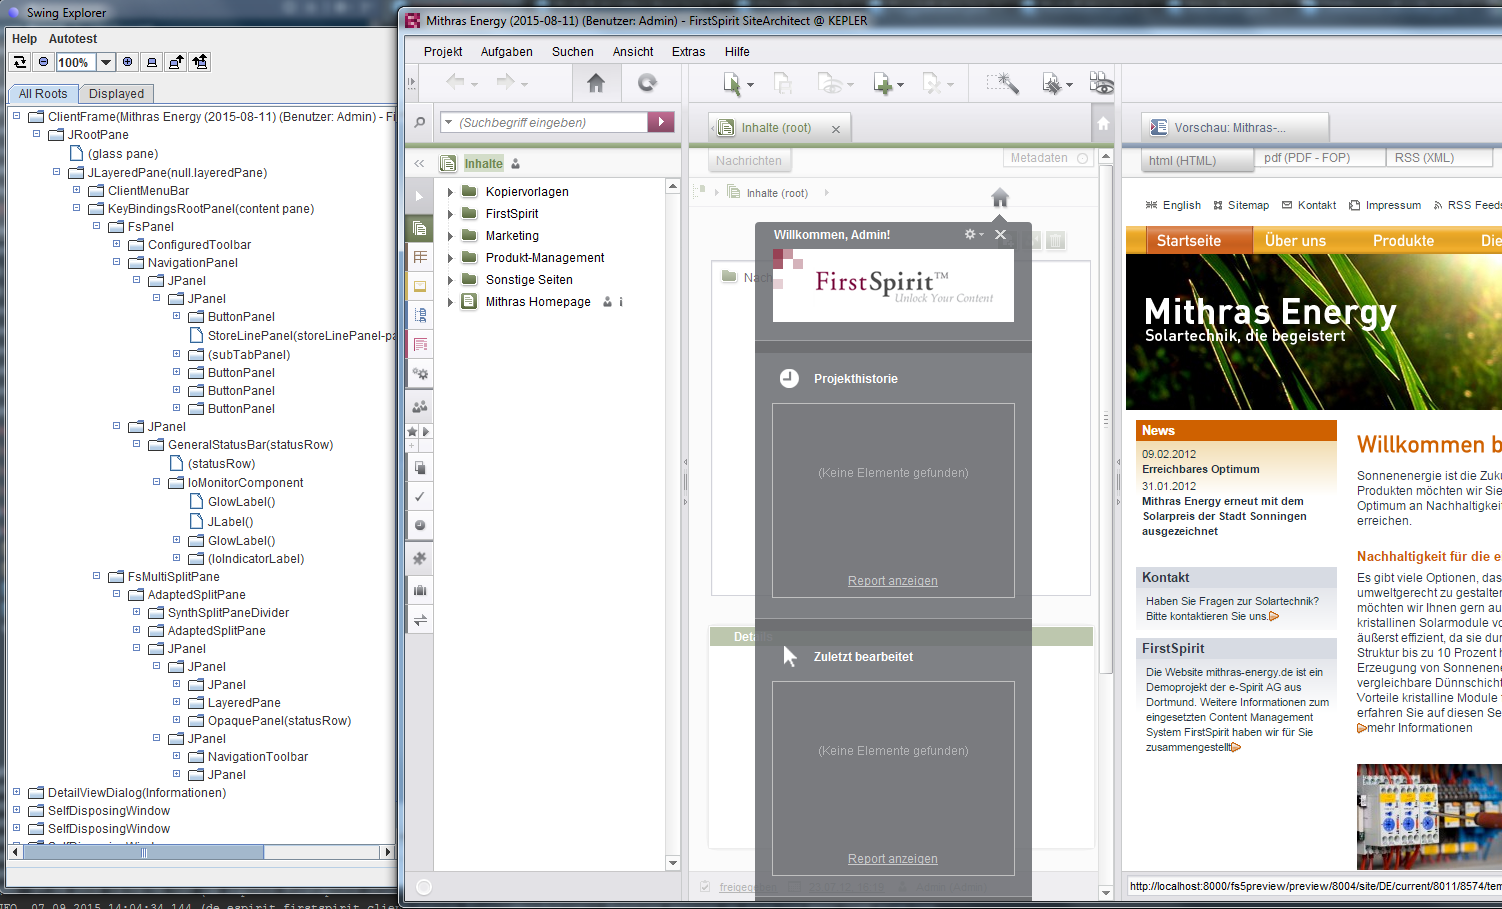
\includegraphics[width=0.85\textwidth]{bilder/screenshot_freespirit.png}
	\caption{Screenshot der e-Spirit CMS-Anwendung FirstSpirit
	sowie anhängigem Swing Explorer, der den Komponentenbaum der Applikation darstellt}
	\label{fig:screenshot_freespirit}
\end{sidewaysfigure}

\begin{figure}
	\centering
	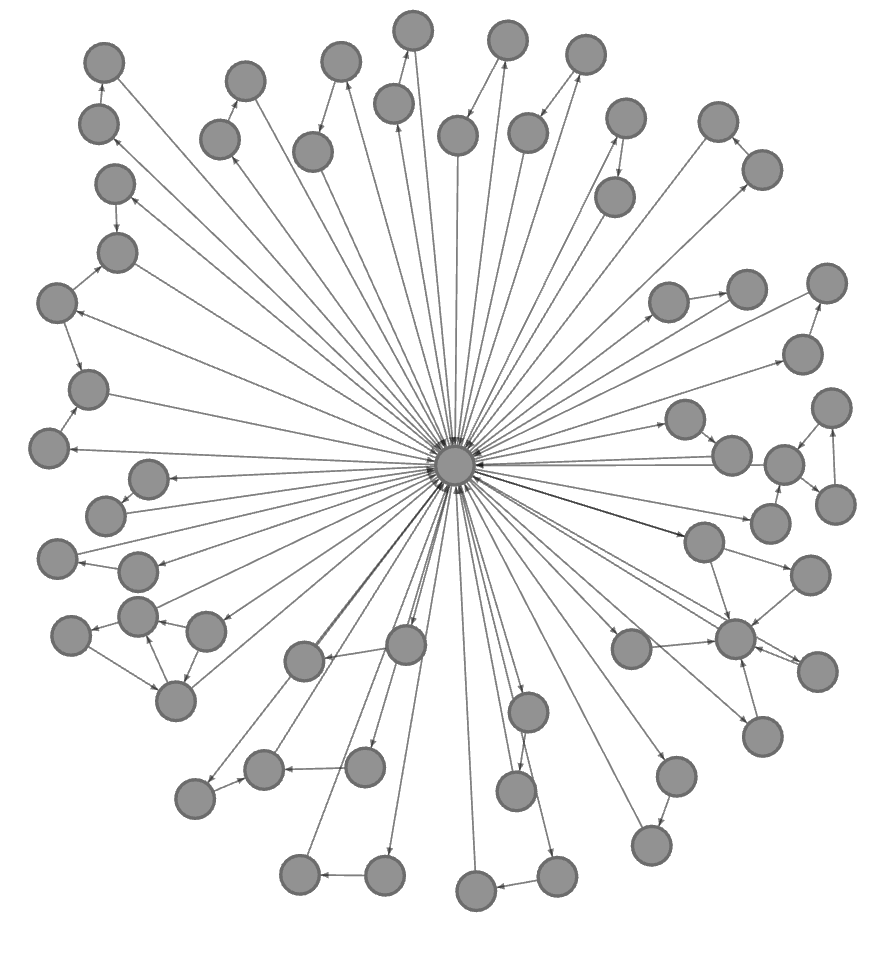
\includegraphics[width=0.85\textwidth]{bilder/model_firstspirit_notext.png}
	\caption{mit Gephi und dem Yifan Hu Algorithmus \cite{hu2005efficient}
    sowie noch für Lesbarkeit maneull angepasste visualierte Graphausgabe 
	des Autotesters über FirstSpirit, hoher Zoomfaktor, keine Beschriftungen.
	Die Pfeile des gerichteten Graphen sind so sichtbar.}
	\label{fig:model_firstspirit_notext}
\end{figure}

\begin{sidewaysfigure}
	\centering
	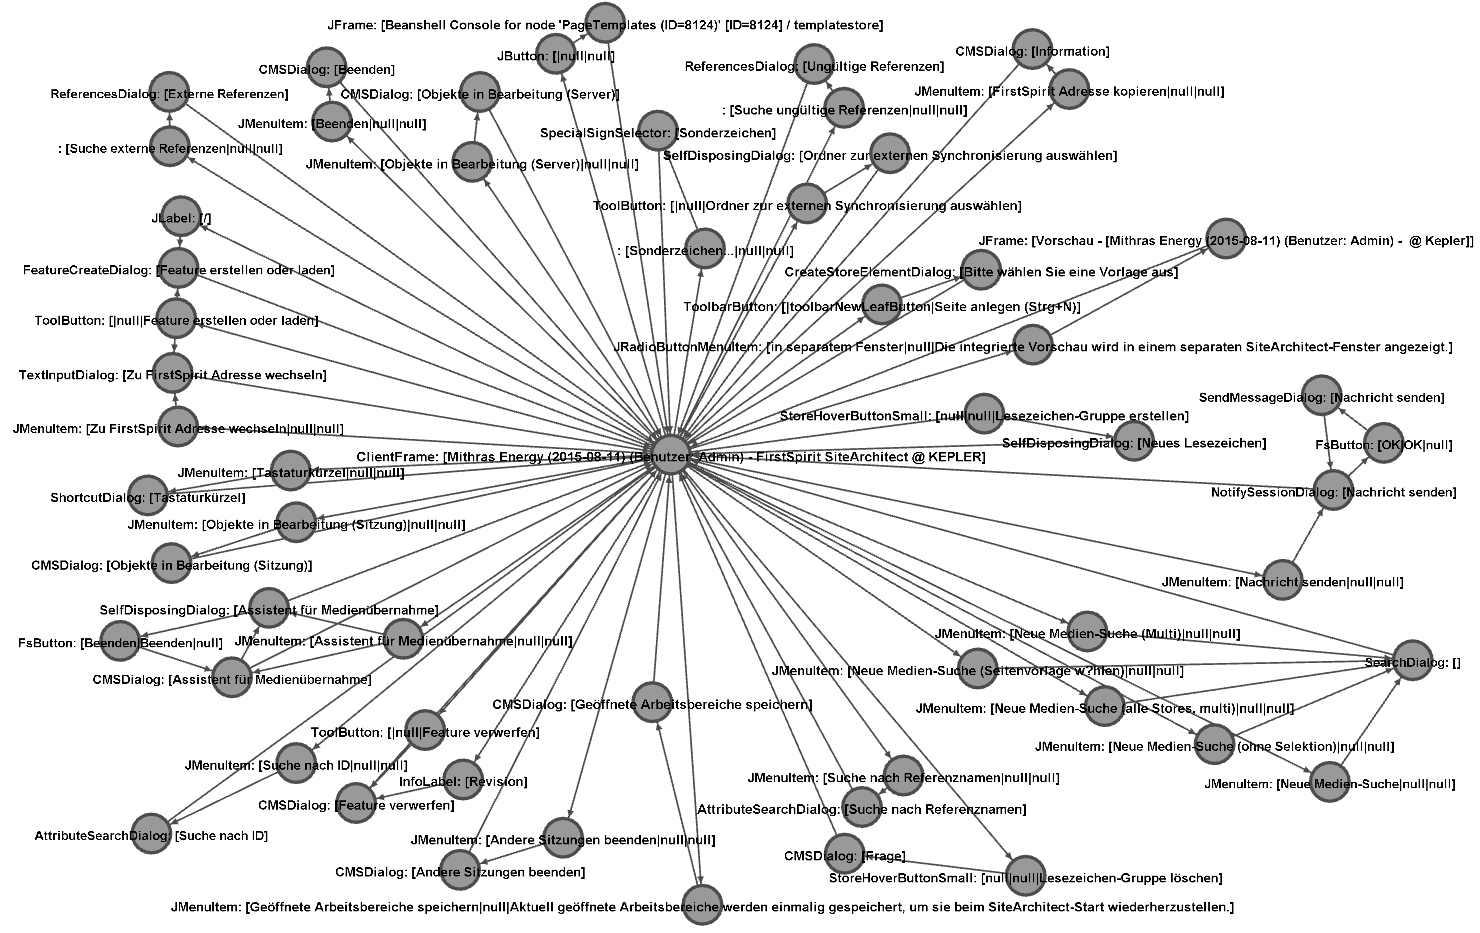
\includegraphics[width=0.85\textwidth]{bilder/model_freespirit.png}
	\caption{mit Gephi und dem Yifan Hu Algorithmus \cite{hu2005efficient}
    sowie noch für Lesbarkeit maneull angepasste visualierte Graphausgabe 
	des Autotesters über FirstSpirit bei einem der ergiebigeren Durchläufe.
	Beschriftungen der Knoten sind deaktiviert.}
	\label{fig:model_freespirit_06.10.2015}
\end{sidewaysfigure}



Die Knoten sind in Dreiergruppen angeordnet: Ein Ursprungsfenster, ein Übergangsknoten
(bzw. ein Wort des Modells), sowie der resultierende Zustand bzw. das sich öffnende Fenster.
Dies ist schlicht eine Frage der Lesbarkeit -- anstelle der mittleren Knoten für Übergänge sollten
eigentlich einfach beschriftete Kanten benutzt werden, aber dies schränkt die Möglichkeiten,
den anhängigen Text in eine lesbare Form zu bringen, zu stark ein. Es ist schlicht zu viel
Textinformation, um mit einer Legende o.Ä. auszukommen.


\section{Vergleich mit klassischen Tests}\label{section:testcomparisonclassic}

